\chapter{Implementation}
\label{ch:impl}

This chapter describes the implementation of \verirego\footnote{
  The tool is available at \url{https://github.com/VeriFIT/VeriRego}.
}, a tool for the verification of \rego access control policies via translation to \smtlib, developed by the VeriFIT research group.
The tool is written in Go, reusing the parsing infrastructure of the Open Policy Agent~\cite{opa:git}.
We describe the architecture of \verirego and the design of its three main components --- the type analysis, the SMT translation, and the policy analyses --- which put into practice the theory established in the preceding chapters.

\section{Architecture}
\label{s:arch}

\verirego{} is structured as a pipeline: a type analysis phase, followed by an SMT
translation phase, whose intermediate output is consumed both by the SMT encoding and
by the policy analyses.
The phases are connected through shared data structures and all operate on the same
parsed representation of the input policy.

\subsection{Pipeline}
\label{ss:pipeline}

The tool accepts a \rego{} policy file as its primary input.
Additionally, the \texttt{input} and \texttt{data} documents --- which the policy is
evaluated against --- can each be provided either as a concrete object (a YAML or JSON
file) or as a symbolic description in the form of a JSON Schema.
Even though both are marked as optional, using such objects in the policy would result in $\Unknown$ values, which are not translatable.

In the type analysis phase, the type map $\typof$ is constructed.
If a concrete or symbolic description of \texttt{input} or \texttt{data} is provided,
the package \texttt{pkg/infer} seeds $\typof$ with the types of their fields before any
policy-level inference takes place.
The package \texttt{pkg/analysis} then traverses the simplified AST and refines $\typof$
according to the inference rules described in Chapter~\ref{ch:typ}.

In the SMT translation phase, the package \texttt{pkg/smt} consumes $\typof$ and the
simplified AST.
The translation begins with two declaration passes: first, the bounded-depth SMT sort
declarations are generated from the inferred types; second, the global variables are
declared.
The policy rules are then parsed into an intermediate representation by \texttt{ParseModule()}, which groups rules by their head variable and translates each rule's bodies into a \texttt{RuleDef} structure.
A \texttt{RuleDef} captures, for each body of a rule: the body condition as an SMT proposition, the assigned value, the local variable bindings, and the source location.
Importantly, \texttt{ParseModule()} does not emit any SMT assertions; it only constructs this structured representation.

From the \texttt{RuleDef} map, two paths are available.
For direct SMT encoding, \texttt{RuleToSmtFromDef()} takes all \texttt{RuleDef}s for a
given head variable and emits the corresponding \smtlib{} assertions.
Because all complete definitions for the same variable are encoded together, this
correctly handles the case of multiple complete rules for the same variable.
For policy analyses, the \texttt{RuleDef} map is consumed directly, without proceeding
to the encoding step.
The resulting \smtlib{} formula can be passed to an SMT solver such as \ziii{} or \cvcv{}.

\begin{figure}
    \centering
    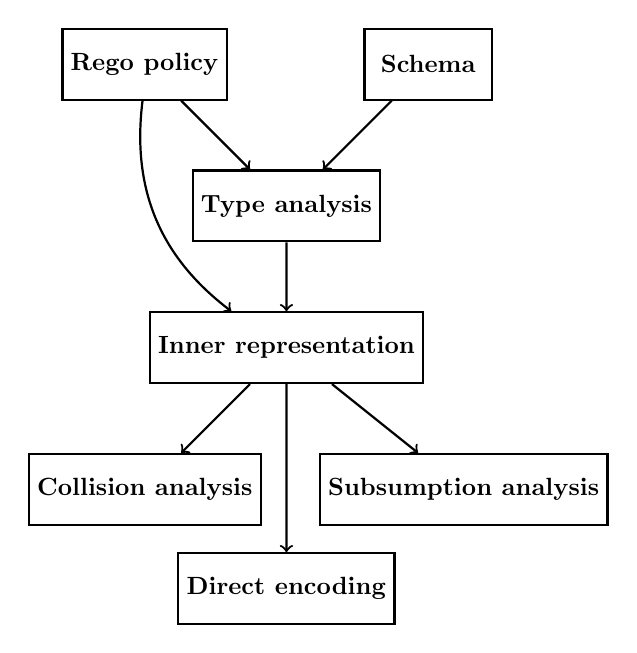
\begin{tikzpicture}[
            s/.style={draw,thick,rectangle,minimum height=10mm, minimum width=18mm},
            % code/.style={draw,fill=blue!10,rectangle,minimum height=10mm, minimum width=18mm,rounded corners=2mm},
            e/.style={fill=gray!50},
            xsh/.style={xshift=15mm},
            transform shape, scale=0.9
        ]

        \tikzset{
            node distance=20mm,
        }

        \node[s] (input) {\textbf{Rego policy}};
        \node[right of=input] (e) {};
        \node[s,right of=e] (schema) {\textbf{Schema}};
        \node[s,below of=e] (ta) {\textbf{Type analysis}};
        \node[s,below of=ta] (ir) {\textbf{Inner representation}};
        \node[below of=ir] (e2) {};
        \node[s,left of=e2] (ca) {\textbf{Collision analysis}};
        \node[s,below of=e2,yshift=6mm] (enc) {\textbf{Direct encoding}};
        \node[s,right of=e2,xshift=5mm] (sa) {\textbf{Subsumption analysis}};

        \draw[->,thick]
            (input) edge (ta)
            (schema) edge (ta)
            (input) edge[bend right] (ir)
            (ta) edge (ir)
            (ir) edge (ca)
            (ir) edge (enc)
            (ir) edge (sa)
        ;

\end{tikzpicture}

    \caption{Data flow through the \verirego{} pipeline.}
    \label{fig:pipeline}
\end{figure}

Each component is also accessible as a standalone command-line tool: \texttt{cmd/type\_analysis}
runs the type analysis and prints the resulting type map, \texttt{cmd/schema\_inference}
infers a JSON Schema from a concrete input document, \texttt{cmd/smt} runs the full
pipeline and outputs the \smtlib{} formula, \texttt{cmd/collision\_analysis} runs the
collision analysis, and \texttt{cmd/subsume\_analysis} runs the subsumption analysis.
This separation allows intermediate results to be inspected and each component to be
tested in isolation.

\subsection{Component interface}
\label{ss:interface}

The coupling between the type analysis and the SMT translation is the \texttt{TypeAnalyzer}
structure, defined in \texttt{pkg/types}.
It holds the type map $\typof$, mapping every Rego term encountered during analysis to
its inferred type, and is the primary output of the type analysis phase.
The SMT translator is instantiated with the \texttt{TypeAnalyzer} and the simplified AST
module as its only inputs, and has no knowledge of how the types were inferred --- only
of the result.

The coupling between the SMT translation and the policy analyses is the \texttt{RuleDef}
map produced by \texttt{ParseModule()}.
The analyses do not depend on the SMT encoding logic; they only require the structured
rule representation.
Conversely, the encoding path via \texttt{RuleToSmtFromDef()} does not depend on any
analysis-specific logic.

The OPA AST module is the shared artifact across all phases: each phase reads the same
parsed representation of the policy, but none modifies it.
As a result, the phases are decoupled in both directions throughout the pipeline.

\section{Type Analysis}
\label{s:ta}

The type analysis component implements the inference described in Chapter~\ref{ch:typ}.
The formal specification there was written to refine the behaviour of the implemented version; minor deviations between the two are noted where they arise.

\subsection{Type Representation}
\label{ss:ta:rep}

The central data structure of the type analysis is the \texttt{TypeAnalyzer}, which
holds the type map $\typof$ as a mutable mapping from Rego term keys to their inferred
types.
Each entry in $\typof$ is represented by a \texttt{RegoTypeDef}, a structure that
encapsulates a single type definition, covering the atomic types ($\Str$, $\Int$,
$\Bool$, $\Null$), array types, object types, union types, and the special $\Unknown$
type.
In the current state of the implementation, we omit the support for sets.

The two operations that mutate $\typof$ during inference correspond to the formal
definitions in Section~\ref{sec:inference}: precision-based update $\refine{v}{\ty}$,
which overwrites an entry only when the new type is strictly more precise, and union
extension $\unionize{v}{\ty}$, which widens an entry into a normalized union.

A key deviation from the formal rules is the treatment of $\Undef$.
In the implementation, $\Undef$ is never written into $\typof$ because types are not deliberately checked for undefined-ness.
This property makes the implementation more straight-forward, but ultimately introduces divergences with the formal specification and the expected behaviour of Rego, and thus is a subject to refinement.

\subsection{Seeding from Input and Data Documents}
\label{ss:ta:seed}

Before policy-level inference begins, $\typof$ is seeded with type information for the \texttt{input} and \texttt{data} documents through the \texttt{InputSchemaAPI} interface, which abstracts over two modes of providing a document.

In the \emph{concrete} mode, a YAML or JSON file containing an actual document is parsed and the types of its fields are read directly from the values present.
In the \emph{symbolic} mode, a JSON Schema is parsed and its declared property types are translated into Rego types, populating the corresponding \texttt{input.*} and \texttt{data.*} paths in $\typof$.
Both modes yield the same result from the perspective of the rest of the pipeline: a partially populated $\typof$ before the policy AST is examined.

As a by-product of this infrastructure, \verirego{} also supports the reverse direction: the \texttt{cmd/schema\_inference} command infers what schema the \texttt{input} document must conform to, by walking the policy and observing how \texttt{input.*} references are used.

\subsection{Policy Inference}
\label{ss:ta:infer}

The main entry point for policy-level inference is \texttt{AnalyzeModule}, which
iterates over the rules of the compiled module and refines $\typof$ for each one.
The traversal is driven by the visitor infrastructure from \texttt{pkg/analysis},
which provides a generic \texttt{ASTVisitor} interface and an \texttt{ASTValueVisitor}
implementation that walks the OPA AST, accumulating and joining a \texttt{PropagatedValue}
across sibling nodes.
The type inference logic is supplied as a concrete instantiation of \texttt{PropagatedValue}.

The visitor methods correspond to the sections of Chapter~\ref{ch:typ}:
\texttt{VisitRule} handles the rule-level structure, \texttt{VisitExpr} corresponds to
the expression inference of Section~\ref{sec:expr-inference}, and \texttt{VisitTerm}
corresponds to the term inference of Section~\ref{sec:term-inference}.
In \texttt{VisitTerm}, the treatment of $\Undef$ follows the deviation described in Section~\ref{ss:ta:rep}: the $\Undef$ type is not accounted for.

\section{Intermediate Representation}
\label{s:ir}

The central output of the SMT translation phase is not an \smtlib{} formula directly,
but an intermediate representation of the policy rules from which both the direct
encoding and the policy analyses are derived (Figure~\ref{fig:pipeline}).
This representation is produced by \texttt{ParseModule()}, which groups all rules of the
module by their head variable and translates each into a \texttt{RuleDef} structure,
yielding a map from head \texttt{SmtValue}s to lists of \texttt{RuleDef}s.

\subsection{Rule and Body Definitions}
\label{ss:ir:repr}

A \texttt{RuleDef} corresponds to a single complete rule in the source policy and holds
its head together with a list of \texttt{BodyDef} structures.
Else-chains are flattened: the else branches are translated recursively and their
\texttt{BodyDef}s appended to the same list, so the entire chain is represented as an
ordered sequence of alternatives.

Each \texttt{BodyDef} captures four things: the body condition as an \texttt{SmtProposition},
the value assigned by the head as an \texttt{SmtValue}, the list of local variable
let-bindings accumulated during body translation, and the source location for
reporting purposes.
Default rules are not represented as \texttt{RuleDef}s; instead, their value is stored
separately and used as the fallback during encoding.

\subsection{Expression Translation}
\label{ss:ir:expr}

The \texttt{ExprTranslator} is the per-rule translation unit, carrying a
\texttt{TransContext} that accumulates local variable bindings throughout the translation
of a single rule body.
Its main entry point, \texttt{BodyToSmt()}, iterates over the expressions of a rule body
and returns a \texttt{SmtProposition} encoding their conjunction together with the list
of local variable let-bindings.

Three cases are handled for each expression.
A single-term expression is converted via \texttt{termToSmtValue()} and its holdability
condition is appended to the conjunction, as described in Section~\ref{ss:expr:val} of
Chapter~\ref{ch:trans}.
A function call in assign form --- detected when the number of supplied arguments exceeds
the declared function arity by one --- is resolved by calling the function on the leading
arguments and recording the result as a let-binding for the trailing return variable.
For the equality operator, the treatment is context-sensitive: if the left-hand variable
has not yet been defined in the current body, the right-hand side is recorded as a
let-binding; otherwise, an equality proposition is appended to the conjunction.

\subsubsection{Reference Navigation}

References of the form \texttt{input.*}, \texttt{data.*}, or \texttt{<package>.<var>}
are resolved by \texttt{refToSmtValue()}, which identifies the base name and the
remaining path, looks up the base type in $\typof$, and delegates to
\texttt{GetSmtRef()} for path navigation.
\texttt{GetSmtRef()} walks the path term by term, dispatching to
\texttt{GetObjSelect()} or \texttt{GetArrSelect()} depending on the current type.

For objects, \texttt{GetObjSelect()} distinguishes three key forms: a constant string
key yields a direct field lookup; a variable key of type $\Str$ yields a dynamic select
over the union of all field types; a reference key is resolved recursively.
For arrays, \texttt{GetArrSelect()} accepts a constant integer index or a variable of
type $\Int$.
At each step, the accessed value is unwrapped from the composite depth to the depth of
the selected element, maintaining sort consistency throughout the navigation.

\subsubsection{Literal Collections}

Constant object and array literals are encoded using the constant-array initialisation
pattern described in Chapter~\ref{ch:trans}.
Both \texttt{objectToSmt()} and \texttt{arrayToSmt()} first look up the type depth of
the literal in $\typof$, initialise a constant array mapping every key to \texttt{OUndef}
at depth $d{-}1$, and then apply a \texttt{store} operation for each key-value pair.
Objects use \texttt{String} as the key sort; arrays use \texttt{Int}.
Each stored value is wrapped to depth $d{-}1$ to match the declared element sort.

\subsection{Direct Encoding}
\label{ss:ir:enc}

The encoding path is taken when the full \smtlib{} formula is required, either for
direct output via \texttt{cmd/smt} or as the base context for the policy analyses.
\texttt{RuleToSmtFromDef()} takes the list of all \texttt{RuleDef}s for a given head
variable and processes them in sequence: for each \texttt{RuleDef}, \texttt{AssertRuleDef()}
emits an \smtlib{} assertion of the form $h = \texttt{ite}(\phi_n, v_n, \ldots
\texttt{ite}(\phi_1, v_1, h)\ldots)$, where the let-bindings of each \texttt{BodyDef}
are wrapped around the corresponding \texttt{ite} in reverse order.

Once all definitions have been asserted, a final fallback assertion is emitted.
It encodes the condition under which no body from any of the rule's definitions applies
and assigns the default value in that case.
Because all complete definitions for the same head variable are processed together,
multiple complete rules for the same variable are handled correctly without any special
casing.

\section{Collision Analysis}
\label{s:impl:collision}

The collision analysis implements the approach described in Section~\ref{s:collision}.
It operates on the \texttt{RuleDef} map produced by \texttt{ParseModule()} and uses
the Z3 SMT solver directly via its Go API\@.
The entry point is \texttt{GetCollisions()}, which takes the translator, the full
\texttt{RuleDef} map, and the name of the rule to analyse.

\subsection{Partial Encoding}
\label{ss:impl:collision:partial}

The first step constructs the partial encoding over the target rule, as defined in
Section~\ref{s:collision}.
The translator's assertion buffer is cleared and the type and variable declarations are
captured as a fixed string \texttt{decls}.
Then, \texttt{RuleToSmtFromDef()} is called for every rule in the map \emph{except} the
target, appending their assertions to the translator.
The resulting formula is loaded into a fresh Z3 solver instance.

Before proceeding, the partial encoding is checked for satisfiability.
If it is unsatisfiable, some other rule already has a collision, and the analysis reports
an error.
This check corresponds to the prerequisite in Section~\ref{s:collision}: the partial
encoding must be satisfiable for any collision in the target rule to be reachable.

\subsection{Class Decomposition}
\label{ss:impl:collision:classes}

With the partial encoding in place, \texttt{splitToClasses()} partitions the
\texttt{RuleDef}s of the target rule into \emph{classes} keyed by the SMT encoding of
their assigned value, directly implementing the $\Class{v}$ construction from
Section~\ref{s:collision}.

For each rule definition and for each body at index $i$ within it, the function
constructs a \texttt{Condition} capturing the proposition that body $i$ \emph{applies}:
all preceding bodies must not hold, and body $i$ must hold.
This is the $\Applies(B_i)$ predicate from Definition~\ref{...}.
If the body's assigned value is a variable rather than a constant, the value is also
stored in the \texttt{Condition} as a \texttt{param} field, marking the class as
requiring the shared-variable treatment.

\subsection{Collision Checking}
\label{ss:impl:collision:check}

\texttt{getCollisions()} iterates over all pairs of distinct classes and calls
\texttt{checkCollision()} for each.

\texttt{checkCollision()} implements the satisfiability query from
Section~\ref{s:collision}.
A fresh SMT variable \texttt{\_\_shared\_\_} is declared at the maximum sort depth of
the two class heads, corresponding to the shared variable $x_{shared}$.
The conditions of each class are then combined into a single proposition by
\texttt{CondsToProp()}: for each \texttt{Condition} in the class, if the assigned value
is a constant (\texttt{param} is nil), the body's proposition is used directly; if the
assigned value is a variable, the proposition is extended with the constraint that the
value equals (for the first class) or does not equal (for the second class)
\texttt{\_\_shared\_\_}.
All per-body propositions within a class are combined with disjunction, reflecting that
any one body applying is sufficient for a collision.

Both resulting propositions are asserted into the solver alongside \texttt{decls} within
a \texttt{Push}/\texttt{Pop} scope, and the solver is queried.
On \textsc{Sat}, the Z3 model is returned and \texttt{inputOfModel()} reconstructs the
concrete input witness from the model's assignments to the \texttt{input.*} variables,
keyed by the field names from the input schema.
On \textsc{Unsat}, no collision exists between those two classes.
